\documentclass[runningheads]{llncs}
\usepackage[T1]{fontenc}
\usepackage{newtxtext}
\usepackage[varvw]{newtxmath}
\usepackage{graphicx}
\usepackage{booktabs}
\usepackage{array}
\usepackage{amsmath}
\usepackage{url}
\usepackage[hidelinks]{hyperref}
\hypersetup{pdftitle={Partial Re-Embedding for Vector Index Migration: An Empirical Study of Quality and Agreement},pdfauthor={Anonymous}}

\begin{document}
\title{Partial Re-Embedding for Vector Index Migration: An Empirical Study of Quality and Agreement}
\titlerunning{Quality and Agreement during Vector Index Migration}
\author{Anonymous Authors}
\authorrunning{Anonymous Authors}
\institute{Anonymous Institution}
\maketitle

\begin{abstract}
Replacing an embedding model changes the representation used by a vector index. Converting existing vectors and gradually replacing them with target embeddings offers a budgeted transition, but agreement with the target ranking need not preserve judged relevance. We study this distinction using three mapping families and four backfill policies, with full-corpus experiments on FiQA and TREC-COVID, additional model transitions, and static and temporal workloads on 50,000-document collections. At approximately 10\% target-vector access on FiQA, degree-prioritized backfill increases top-10 agreement from 0.3866 to 0.4057 relative to random backfill, while nDCG@10 decreases from 0.2800 to 0.2332. The old-model system achieves 0.3687 nDCG@10, showing that early migration can lose relevance even when the fully migrated model is better. Coverage-greedy selection has sparse positive gains in several workloads and does not consistently outperform simpler policies. Read-prioritized backfill improves agreement in the observed temporal replay, with limited evidence about relevance. These results support evaluating partial migration through separate relevance and agreement curves, explicit access accounting, and the scheduling signal available in each workload.
\keywords{Vector retrieval \and Embedding migration \and Partial re-embedding \and Retrieval evaluation}
\end{abstract}

\section{Introduction}

Dense retrieval represents documents and queries in a shared embedding space. When an encoder is replaced, its output can differ in dimension, geometry, normalization, and task behavior. An existing document index therefore cannot generally serve queries from the replacement encoder without adaptation. Computing target embeddings for the entire collection provides a direct transition, but requires access to every document through the target encoder. A collection owner with a restricted transition budget must decide what to serve before that process finishes.

One approach converts old document embeddings into the target space and gradually replaces converted vectors with actual target embeddings. Query-side adaptation provides another option by mapping target queries into the old document space. Both directions have been studied: Drift-Adapter investigates query adaptation for model upgrades~\cite{vejendla-2025-drift}, and Embedding-Converter studies cross-model transformation, including retrieval with a mixture of converted and true embeddings~\cite{yoon-arik-2025-embedding}. The existence of a mixed representation is consequently a starting point for this study.

The practical question is whether a partially migrated collection offers useful retrieval at a particular budget. Two evaluation goals arise. Agreement measures how closely a transitional system reproduces the fully migrated target ranking. Relevance measures whether its results satisfy external relevance judgments. These goals are related through retrieval behavior, but they are not interchangeable. The target model is a reference system rather than a relevance oracle. Even when it improves aggregate relevance over the old model, a transition that more closely imitates its top-10 sets can have worse relevance than another transition.

Our FiQA results illustrate the consequence for choosing which documents to replace. At approximately 10\% total target-document access, degree prioritization improves top-10 agreement over random replacement by 0.0191, but reduces nDCG@10 by 0.0468. Moreover, random replacement with the residual-MLP pipeline achieves 0.2800 nDCG@10, compared with 0.3687 for the old-model system and 0.4996 for the full target system. Thus a favorable full-model comparison does not establish that an early query-encoder cutover is useful.

We investigate three questions. \textbf{RQ1:} How do relevance and agreement evolve with the target-vector budget, and how do mapping families compare? \textbf{RQ2:} How do random, degree, read-prioritized, and coverage-greedy backfill differ under common migration settings? \textbf{RQ3:} How do the observed behaviors vary with model transition, workload scope, and available scheduling signal? We use FiQA as the principal controlled comparison, TREC-COVID as an additional full-corpus mapping comparison, and explicitly bounded supporting cases for larger collections and temporal traffic.

The study makes three empirical contributions. First, it presents relevance and agreement curves that account for bootstrap access and subsequent backfill. Second, it quantifies policy ranking reversals and early relevance degradation under common controls. Third, it examines selection activity across workloads, identifying cases where coverage selection has few or no positive gains. These findings concern the evaluated pipelines and populations; causal explanations require further component studies.

\section{Background and Related Work}

\subsection{Adapting Representations across Models}

Frozen-encoder adaptation learns a transformation between embeddings without retraining the original encoders. The direction matters. A query-to-old-space adapter retains the old document representation and changes incoming query vectors. A document-to-target-space converter changes the stored representation and enables direct use of target query embeddings. These alternatives incur different access, storage, and eventual replacement requirements.

Drift-Adapter~\cite{vejendla-2025-drift} studies query-side adaptation using orthogonal, affine, and nonlinear transformations. Our forward document transformations use related mapping families but have a different orientation and training budget. They are not a reproduction of that method. Embedding-Converter~\cite{yoon-arik-2025-embedding} proposes a cross-model conversion framework. Its Appendix D.3, Tables 13--14, already evaluates mixtures containing 50\% converted and 50\% true embeddings. We therefore locate our contribution in the measured transition curves and policy behavior, rather than in introducing mixed embeddings.

Recent alignment work also studies the geometry that permits transformations across embedding spaces. Procrustes analyses~\cite{procrustes} and linear geometry alignment~\cite{minivec} provide related perspectives on compatibility. Geometric approximation and retrieval evaluation answer different questions: a lower vector prediction loss or stronger set overlap does not by itself establish better externally judged relevance. In our experiments, mapping comparisons include a common local correction and scoring procedure, so their results describe complete mapping-based pipelines rather than isolated global-map effects.

\subsection{Selective Updates and Index Migration}

Selective document replacement can use graph connectivity, retrieval activity, or a proxy for expected benefit. The usefulness of these signals depends on which queries are available and how their associated documents overlap the indexed collection. Static click relations and chronological request histories also support different claims about future queries.

Embedding Surgery~\cite{surgery} investigates localized embedding updates for ranking correction. Cross-model graph migration~\cite{graphmigration} studies reuse of graph structure during index construction. These problems are relevant to maintaining retrieval systems as representations change, but they differ from allocating a restricted budget of target-document vector accesses. In particular, improving graph construction with target vectors already available does not establish how relevance behaves while most target vectors remain unavailable to the migration procedure.

HNSW~\cite{hnsw} introduces an additional approximation layer. We separate its fidelity to a stored-vector snapshot from agreement with the fully migrated target. A highly faithful approximate index can serve a mixed snapshot accurately while that snapshot has poor target agreement or poor relevance. Our principal relevance comparisons use exact search to avoid conflating these effects.

\section{Problem and Migration Procedure}

\subsection{Mixed Representation and Access Budget}

Let a collection contain $N$ documents. Document $i$ has an old normalized embedding $x_i\in\mathbb{R}^{d_o}$ and a target normalized embedding $y_i\in\mathbb{R}^{d_t}$. Let $A$ be the set of documents whose target vectors have been accessed by the migration procedure. A forward map $M_0$ and a region-specific affine correction produce a replacement for each remaining old vector:
\begin{equation}
 z_i=\begin{cases}
 y_i, & i\in A,\\
 \operatorname{norm}(A_{r(i)}M_0(x_i)+c_{r(i)}), & i\notin A.
 \end{cases}
 \label{eq:mixed}
\end{equation}
Here $r(i)$ is a region assignment determined from old embeddings. The target query encoder produces a normalized vector $q$. The index stores one current vector per document and a flag indicating whether it is a true target vector.

The budget is $b=|A|/N$, counting unique target-document accesses. It includes training, validation, calibration, and subsequently selected backfill documents. All accessed bootstrap vectors also enter the served index as true vectors. We separately track the incremental backfilled fraction. An independent evaluator can access the full target representation to construct references; its access is excluded from the simulated migration budget. Thus $b$ measures information available to the migration procedure, not the total computation used to create the experimental caches.

\begin{figure}[t]
\centering
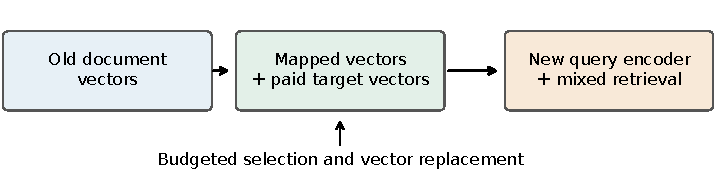
\includegraphics[width=\linewidth]{figures/procedure.pdf}
\caption{The evaluated transition. Accessed bootstrap and backfill vectors replace mapped document vectors; queries use the target encoder. The access budget counts both sources of true vectors.}
\label{fig:procedure}
\end{figure}

\subsection{Mapping and Scoring}

We evaluate orthogonal Procrustes (OP), low-rank affine (LA), and residual-MLP global maps. OP is fitted by singular value decomposition, with zero padding for unequal dimensions. LA has rank 64. The MLP adds a width-256 GELU residual branch to an OP-initialized linear branch; its last residual layer is initialized to zero. The trainable maps minimize squared prediction error before output normalization, using Adam and validation-based selection from learning rates $10^{-4}$ and $10^{-3}$, with at most 50 epochs and patience five. Neither document encoder is fine-tuned.

The bootstrap training pool contains $\min(10{,}000,\lceil0.02N\rceil)$ documents. Validation contains $\min(2{,}000,\lceil0.005N\rceil)$ documents; each calibration document pool has a cap of $\min(1{,}000,\lceil0.005N\rceil)$. Pools are disjoint. Calibration documents are proposed using a common OP retrieval procedure in the principal mapping comparison, so candidate construction is shared across the mapping variants. Actual pool occupancy determines the charged bootstrap budget.

Old-space mini-batch clustering fixes the region assignments. The region count is the largest power of two not exceeding $\min(256,\max(1,\lfloor n_{\mathrm{train}}/100\rfloor))$: eight on FiQA and the 50k cases, and 32 on TREC-COVID. Within a region, ridge regression fits an affine correction to global-map outputs, with regularization 10 toward the identity transformation. Regions with fewer than 20 paired observations retain the identity correction. The global map and assignments remain fixed, while regional corrections are refitted after each additional 5\% of collection-sized backfill. Remaining mapped vectors in affected regions are then updated.

Mapped and true scores can have different distributions. For mapped documents, positive affine calibration transforms the raw dot product as $a(q^\top z_i)+c$, with $a\geq10^{-6}$; true documents retain $q^\top y_i$. Calibration-fit and calibration-check query groups are disjoint. The latter provide a 95th-percentile absolute score-residual radius $\rho$. Insufficient calibration data lead to identity scoring or an unavailable radius. This empirical radius characterizes the observed calibration population and supplies a selection proxy; it is not a simultaneous ranking certificate.

\subsection{Backfill Policies}

All policies select only documents not already in $A$, obey the same access target, and share the update procedure. Batches contain at most 1\% of the collection and stop at the next checkpoint or regional-refit boundary.

\textbf{Random} samples from the remaining mapped documents. \textbf{Degree} prioritizes the number of unique scheduling-query neighbors attached to each document, with deterministic document-ID ties. \textbf{Read-prioritized} traverses top-10 retrieval results in a fixed development-query order and replaces encountered mapped documents. It retains a cursor and pending results between batches, then uses random selection if the list is exhausted. This is retrieval-driven selection over a specified order, rather than a measurement of live request-triggered inference.

\textbf{Coverage-greedy} constructs a weighted fixed-snapshot coverage objective. For a scheduling query, let the slack of a current top-10 result be its score minus the score of the eleventh result. Proxy-associated mapped documents are eligible when their slack is in $(\rho,2\rho]$. A query with a proxy result beyond $2\rho$ is excluded by the implemented safety heuristic. The proxy is drawn from available training/click associations, with retrieval results used where that proxy is unavailable. Greedy selection covers remaining weighted query sets while marginal gain is positive. After positive gain is exhausted, random selection fills the batch. Missing or nonpositive radius yields no positive-gain candidates.

This snapshot objective does not optimize judged nDCG directly. Retrieval, refitting, and calibration can change its candidate sets. We report positive-gain and fallback counts to distinguish active prioritization from random fill.

\section{Experimental Design}

\subsection{Collections and Model Transitions}

Table~\ref{tab:data} summarizes the evaluated populations. FiQA and TREC-COVID use their full document collections and external test judgments from BEIR~\cite{beir}. FiQA has 648 test queries and disjoint development roles: 4,400 scheduling queries, 500 tuning queries, and 550 queries in each calibration role. TREC-COVID has 50 test queries and no independent scheduling query set in this study, so its principal experiment compares mappings under random replacement.

\begin{table}[t]
\caption{Evaluated collection sizes and query populations. A 50k collection is a reduced corpus. Supporting cases use agreement when the reduced corpus retains too few positive judgments for a standard relevance comparison.}
\label{tab:data}
\centering
\small
\setlength{\tabcolsep}{3pt}
\begin{tabular}{@{}lrr>{\raggedright\arraybackslash}p{4.7cm}@{}}
\toprule
Collection & Documents & Eval queries & Evaluation scope \\
\midrule
FiQA & 57,638 & 648 & Held-out test; full collection \\
TREC-COVID & 171,332 & 50 & Held-out test; mapping comparison \\
NQ & 50,000 & 500 & Reduced corpus; no scheduling set \\
HotpotQA & 50,000 & 500 & Reduced corpus; development scheduling \\
FEVER & 50,000 & 500 & Reduced corpus; development scheduling \\
MS MARCO docs & 50,000 & 5,000 & Same ORCAS queries used for scheduling \\
AOL-IA & 50,000 & 50,000 rows/week & Seven future-week evaluations \\
\bottomrule
\end{tabular}
\end{table}

The main transition is all-MiniLM-L6-v2 to all-mpnet-base-v2~\cite{minilm}, with dimensions 384 and 768 and token limits 256 and 384. Additional transitions are Arctic embed-l to embed-l-v2.0~\cite{arctic} (1024 to 1024; token limits 512 to 8192), Nomic text-v1 to v1.5~\cite{nomic} (768 to 768; both 8192), and BGE base-en-v1.5 to M3~\cite{bge} (768 to 1024; 512 to 8192). The evaluated configuration uses normalized dense float32 vectors and the prescribed query/document prefixes for each encoder. The BGE comparison uses dense vectors. These are complete encoder transitions, including preprocessing differences, rather than controlled changes in geometry alone.

The additional static cases are listed in Table~\ref{tab:cases}. Reduced document pools use uniform sampling based on document hashes. Only 4--14 of 500 queries retain a positive judgment in the NQ, HotpotQA, and FEVER pools. Their agreement provides supporting evidence, while their nDCG cannot represent standard full-corpus BEIR performance. Query samples also differ between model-pair cases for NQ and FEVER.

The static workload experiment uses a 50,000-document subset of MS MARCO document ranking v1 and 5,000 ORCAS query groups~\cite{orcas}. ORCAS provides static clicked query--document relations, not chronological traffic frequencies; query groups have uniform weight here. Only 137 of these groups have a clicked edge into the selected document pool. Evaluation uses the same groups that guide scheduling, so its result estimates agreement on a known workload. The available held-out ORCAS groups are not evaluated in this comparison.

The temporal case evaluates AOL-IA~\cite{aol} using 50,000 recovered documents. Eight selected weeks span 1 March--25 April 2006, with 50,000 log rows per week. Seven decisions use past-week information before evaluating the next week. A query can have multiple clicked-item rows; weighting follows this selected row population. Public metadata omit query and document text, limiting independent encoder-level reconstruction.

\subsection{Controls, Search, and Budgets}

FiQA compares the three mapping pipelines under random backfill and the four policies under the residual-MLP pipeline. It uses mapping seeds 17, 29, and 43 with one traffic order, seed 101. The residual-MLP/random cells shared by the two comparisons are identical and are counted once for statistical inference. TREC-COVID and the additional static model-pair cases have one mapping seed. MS MARCO uses the same three mapping seeds; the temporal replay uses one.

The static checkpoints are bootstrap, approximately 5\%, 10\%, 25\%, 50\%, and complete target-vector access. Integer document counts determine the actual fractions. FiQA bootstrap accesses 2,020 documents; its nominal 10\% checkpoint accesses 5,763 documents, including 3,743 subsequent backfill documents. TREC-COVID starts with 4,284 accesses. MS MARCO starts with 1,750 and reaches 5,000 at 10\%, including 3,250 incremental replacements.

The temporal replay uses smaller successive allocations. Its final accessed count is 3,501 of 50,000 documents (7.002\%), including 1,750 bootstrap and 1,751 backfill documents. This is the realized budget of the evaluated replay. Query embeddings are precomputed for evaluation, while scheduling filters history by its allowed time window; the experiment measures chronological selection rather than live encoder execution.

The principal static quality comparisons and additional model-pair cases use exact search. The MS MARCO experiment uses HNSW with $M=16$, construction parameter 200, 1,000 retrieved candidates, search parameter 2,000, and eight search threads. Exact target rankings define agreement. HNSW fidelity is evaluated separately against exact search over the same stored-vector snapshot. Vector updates preserve document IDs; the implementation can rebuild the graph after an index-query failure. Cached execution times include selection and maintenance but do not isolate target inference or establish production latency.

\subsection{Metrics and Uncertainty}

For a query $q$, let $T_{10}(q)$ be the exact full-target top-10 set and $S_{10}(q)$ the evaluated top-10 set. We define
\begin{equation}
 \mathrm{ARR@10}(q)=\frac{|S_{10}(q)\cap T_{10}(q)|}{10}.
\end{equation}
ARR is a set-agreement measure and ignores ordering within the intersection. Judged nDCG@10 uses the evaluator's linear relevance gains. Hit@10 records any judged-relevant result in the top 10. NFR@1 records queries for which the target top-1 is relevant and the evaluated top-1 is not, divided by all evaluation queries. Old/old retrieval uses the old query and document encoders; full-new retrieval uses the target pair. Neither reference is assumed to dominate judged relevance on every collection.

For FiQA, we average each query's outcome across the three mapping seeds before paired analysis, using 10,000 bootstrap draws for conditional 95\% confidence intervals. We report three Greedy-versus-baseline contrasts with sign-flip tests and Holm adjustment within each metric. These reanalyses are exploratory. Intervals condition on the evaluated seed grid and do not quantify arbitrary retraining or workload variation. MS MARCO provides aggregate results only, so we report seed ranges without query-level significance claims.

AOL estimates are weighted by selected log rows. The bootstrap resamples users, retaining dependence among their rows. The final week contains 4,563 users and 23,629 query groups. An exploratory paired bootstrap compares Read and Random on this population. The selected weeks form one chronology.

\section{Results}

\subsection{RQ1: Relevance during Partial Replacement}

\begin{figure}[t]
\centering
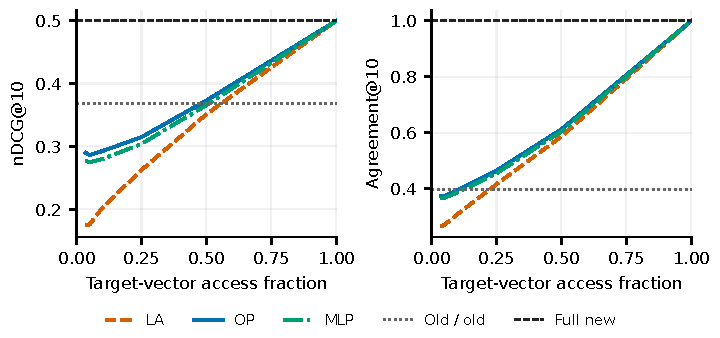
\includegraphics[width=\linewidth]{figures/mapping_curves.pdf}
\caption{FiQA mapping pipelines under random backfill. Lines are means across three mapping seeds; shading is the seed min--max range. Horizontal lines show old/old and full-new references. Curves start at the charged bootstrap budget.}
\label{fig:mapping}
\end{figure}

Figure~\ref{fig:mapping} shows that agreement and relevance evolve differently during migration. At approximately 10\% access, FiQA OP achieves mean nDCG@10 of 0.2928, residual MLP 0.2800, and LA 0.2029. All are below the old-model reference of 0.3687, despite the full-target reference reaching 0.4996. For residual MLP, the exploratory paired difference from old/old is $-0.0887$, with a query-bootstrap interval of $[-0.1094,-0.0687]$. This observed early quality loss directly affects whether switching the query encoder is beneficial under a small budget.

More target access improves the broad trajectory, but the measured curves need not be monotone at every checkpoint. At 50\% access, residual-MLP/random mean nDCG is 0.3657, close to the old reference; its paired difference remains unresolved. OP first exceeds the old mean at the observed 50\% checkpoint. The measured grid does not identify an exact break-even access threshold between checkpoints. At complete access, exact retrieval equals the target reference for all compared static configurations.

On TREC-COVID, residual MLP reaches 0.4503 nDCG@10 at approximately 10\% access, OP 0.4412, and LA 0.4094, compared with old/old at 0.4721 and full-new at 0.5132. OP's FiQA advantage therefore does not establish a universally preferable mapping family. FiQA has three seeds and 648 queries, whereas TREC-COVID has one seed and 50 queries.

These comparisons concern the global-map family inside the common regional and calibration procedure. They do not isolate whether global prediction error, local correction, or cross-fidelity score calibration causes the quality differences. The lower MLP vector-validation error observed during tuning is insufficient to predict the ordering of judged retrieval results. A controlled component study would be needed to attribute the early degradation to a particular operation.

\subsection{RQ2: Agreement and Relevance Favor Different Policies}

\begin{table}[t]
\caption{FiQA at 5,763/57,638 target-document accesses, residual-MLP pipeline. Values are means over three mapping seeds. The bracketed nDCG values are seed ranges, not confidence intervals. NFR uses all 648 test queries as its denominator.}
\label{tab:policies}
\centering
\small
\begin{tabular*}{\linewidth}{@{\extracolsep{\fill}}lrrrrr@{}}
\toprule
Policy & nDCG@10 & Seed range & ARR@10 & Hit@10 & NFR@1 \\
\midrule
Random & 0.2800 & [0.2799, 0.2801] & 0.3866 & 0.5905 & 0.2994 \\
Degree & 0.2332 & [0.2320, 0.2351] & 0.4057 & 0.5391 & 0.3416 \\
Read & 0.2806 & [0.2789, 0.2818] & 0.4170 & 0.5977 & 0.2886 \\
Greedy & 0.2779 & [0.2728, 0.2835] & 0.3861 & 0.5931 & 0.3086 \\
\bottomrule
\end{tabular*}
\end{table}

Table~\ref{tab:policies} compares the four backfill policies under a common mapping pipeline. Degree has higher agreement than Random, 0.4057 versus 0.3866, while its judged nDCG is substantially lower, 0.2332 versus 0.2800. Read obtains the highest agreement of these policies, 0.4170, while its nDCG of 0.2806 is close to Random. Consequently, a policy choice based only on target top-10 overlap would hide a material relevance difference.

\begin{figure}[t]
\centering
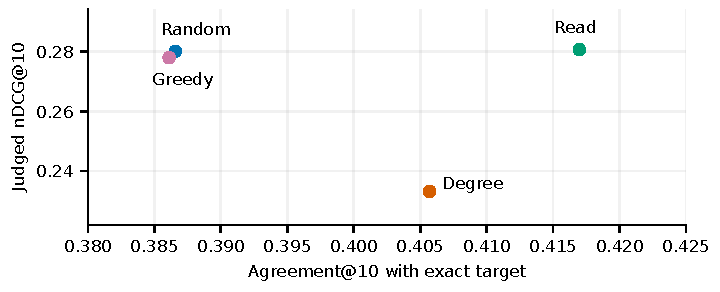
\includegraphics[width=\linewidth]{figures/policy_tradeoff.pdf}
\caption{FiQA policy means at approximately 10\% target-vector access. Agreement and judged relevance give different policy orderings. The plot shows aggregate points; paired uncertainty is discussed in the text.}
\label{fig:tradeoff}
\end{figure}

Greedy reaches 0.2779 nDCG and 0.3861 agreement. Its nDCG difference from Random is $-0.0021$, with conditional 95\% CI $[-0.0126,0.0082]$; the corresponding difference from Read is $-0.0027$, CI $[-0.0161,0.0105]$. These estimates do not resolve an advantage for Greedy and do not establish equivalence. Greedy exceeds Degree in nDCG by 0.0447, CI $[0.0363,0.0534]$, while its agreement is lower by 0.0196, CI $[-0.0276,-0.0119]$. The two metrics reverse the direction of this contrast.

For agreement, Greedy--Read is $-0.0309$, with CI $[-0.0392,-0.0225]$, whereas Greedy--Random is $-0.0005$, CI $[-0.0062,0.0052]$. The Greedy--Degree and Greedy--Read agreement contrasts, and the Greedy--Degree nDCG contrast, each have Holm-adjusted sign-flip $p\approx0.0003$ within their respective contrast families. The study therefore supports specific disagreements between policy rankings, rather than a claim that one policy improves all retrieval objectives.

The result is not surprising from the definitions alone: judged relevance and target set overlap have different references. Its practical significance lies in the measured size of the loss and the fact that it occurs while the full target model has better overall relevance than the old model. Agreement is useful for measuring convergence toward a target representation, but it does not suffice for selecting an early migration state or a backfill policy.

\subsection{RQ3: Workload Scope and Available Selection Signal}

\begin{figure}[t]
\centering
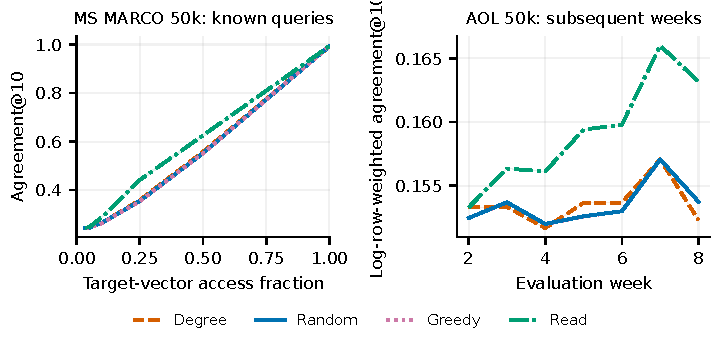
\includegraphics[width=\linewidth]{figures/workload_curves.pdf}
\caption{Agreement on a known static workload and subsequent temporal weeks. MS MARCO shading is the range across three mapping seeds; AOL lines use one chronology and log-row weights. Random and Greedy coincide in the temporal replay. The two panels have different budgets and evaluation populations.}
\label{fig:workloads}
\end{figure}

\textbf{Known static queries.} At 10\% target access on MS MARCO50k, Read achieves mean agreement 0.2883, Random 0.2657, Degree 0.2647, and Greedy 0.2635. Read's advantage over Random is 0.0227 on the evaluated query groups. Because these are also the scheduling groups, this comparison measures within-workload effectiveness. It provides no direct estimate of held-out query generalization, and aggregate-only output prevents a query-level paired uncertainty analysis.

The positive-gain mechanism in Greedy is rarely active. Across its three seeds, only 18--20 of the 3,250 backfill documents selected by 10\% access are chosen through positive coverage gain. The rest are random fills. By completion, its positive-gain counts remain 22, 22, and 24 out of 48,250 incremental replacements. These counts explain why the nominal policy cannot be interpreted as sustained greedy prioritization over the full transition. Sparse clicked-edge overlap is one relevant property of the setting, but the present design does not isolate it as the cause of gain exhaustion.

At complete replacement, the actual HNSW-served agreement ranges from 0.9915 to 0.9953 across the 12 static workload configurations. A separately constructed exact target reference agrees with itself at 1.0. Those are distinct measurements: completing vector replacement does not remove approximate-search error from the serving graph. We retain the observed approximate endpoints rather than forcing each curve to end at one.

\textbf{Temporal replay.} In the final AOL week, weighted agreement is 0.163158 for Read, 0.153740 for Random and Greedy, and 0.152308 for Degree. The exploratory paired Read--Random difference is 0.009418. Bootstrap resampling by user gives a 95\% interval of $[0.006696,0.012306]$. This supports an agreement benefit on the selected future-week population. Judged relevance is not reported for this reduced document pool.

All 1,751 Greedy backfill selections in the temporal replay are fallback selections. Its identity with Random therefore evaluates the shared fallback realization, rather than two effective prioritization mechanisms with equal performance. Read uses history-derived query lists in group-ID order, retaining its cursor as those lists change; the implementation does not replay every historical query as a live request in its original arrival order. This distinction limits the deployment interpretation of its measured advantage.

Only 8,971 of 216,723 selected clicked rows refer to documents in the temporal pool, approximately 4.14\%. Recovery coverage, corpus truncation, and log-row sampling all affect the population. The temporal result is consequently a bounded case study of past-informed selection, with one model transition and one selected chronology.

\subsection{Variation across Model Transitions}

\begin{table}[t]
\caption{Additional static cases at approximately 10\% access. M--P denotes MiniLM--MPNet; R and G denote residual-MLP Random and Greedy. Coverage is the percentage of evaluation queries retaining a positive qrel in the evaluated corpus. ``No'' means no independent scheduling queries; the G result is then fallback. OP is an additional greedy-policy cross-check where available. Each row uses one seed.}
\label{tab:cases}
\centering
\small
\setlength{\tabcolsep}{3pt}
\begin{tabular}{@{}lrrlrrr@{}}
\toprule
Collection / transition & Docs & Coverage & Schedule & R ARR & G ARR & OP ARR \\
\midrule
FiQA / M--P & 57,638 & 100\% & Yes & .3852 & .3878 & .3938 \\
TREC / M--P & 171,332 & 100\% & No & .4680 & .4680 & -- \\
NQ / Arctic & 50,000 & 2.4\% & No & .3810 & .3810 & .3622 \\
HotpotQA / Arctic & 50,000 & 1.6\% & Yes & .2670 & .2742 & -- \\
FEVER / Nomic & 50,000 & 0.8\% & Yes & .7208 & .7208 & .6976 \\
FiQA / Nomic & 57,638 & 100\% & Yes & .7535 & .7568 & -- \\
NQ / BGE & 50,000 & 2.8\% & No & .2970 & .2970 & -- \\
FEVER / BGE & 50,000 & 1.4\% & Yes & .2270 & .2236 & .2148 \\
\bottomrule
\end{tabular}
\end{table}

Table~\ref{tab:cases} shows substantial variation in partial-migration agreement. FiQA/Nomic reaches 0.7535 with Random at 10\%, compared with roughly 0.3866 in the principal MiniLM--MPNet comparison. On the reduced FEVER cases, Nomic agreement is 0.7208 while BGE is approximately 0.2270. The document pools, query samples, and complete encoder configurations are not held identical across all cases, so these values cannot isolate model drift as a causal variable. They show that a single reported migration curve is not representative of every transition.

High agreement also need not imply that the target model improves relevance. For full FiQA under Nomic, old/old nDCG is 0.3802 and full-new is 0.3765. Their exploratory paired difference is $-0.0037$, with CI $[-0.0143,0.0068]$. This comparison does not resolve a target relevance gain. At 10\%, Random nDCG is 0.3640 and Greedy 0.3606, despite their agreement being relatively high. The baseline relevance of the proposed target must therefore be checked independently of the ease of approximating its ranking.

The additional cases also reveal a policy-availability issue. TREC-COVID and the two NQ cases lack scheduling queries, so their Greedy runs reduce to random fallback and produce equal outcomes. Among cases with scheduling queries, the Greedy--Random agreement difference can be positive, zero, or negative. These observations support reporting the presence and use of scheduling signal, rather than treating all labeled policy runs as equally informative tests of the coverage objective.

\subsection{Index Fidelity and Maintenance Scope}

Supporting HNSW probes on FiQA use a fully target-vector snapshot and 1,600 development queries combining tuning and calibration roles. Fixed-snapshot serving recall against exact stored-vector search is 0.9991. Small same-ID update probes perturb vectors by Gaussian noise of scale $10^{-5}$; their serving fidelity remains above 0.998 at the measured checks. These probes test a local update path and do not compare relevance under alternative regional-refit cadences.

A separate 50,000-document bootstrap probe has serving recall 0.996875, graph footprint about 399.3\,MiB, and peak process memory about 8.90\,GiB. It disables score calibration for that probe. Across the 12 static workload migrations, the stored counters record 22 graph rebuilds by completion. The index implementation therefore includes a recovery cost that must be considered when interpreting cached execution times. The probes establish fidelity in their measured states; they do not establish production tail latency, downtime, or end-to-end target-encoder savings.

\section{Discussion and Limitations}

\textbf{Evaluate the cutover decision.} A target model with better full-corpus relevance can still produce a poor transitional system when most stored vectors are mapped. The observed FiQA gap motivates comparing each partial state with old/old retrieval, not only normalizing its score by the full-target result. The first observed checkpoint exceeding old quality is useful descriptive information, but a coarse checkpoint grid cannot establish an exact minimum deployment budget.

\textbf{Keep objectives separate.} Agreement characterizes convergence to a target ranking. Judged relevance characterizes usefulness under external labels. Their policy-ranking reversal makes a single combined ``quality'' score difficult to interpret. An operator concerned about user relevance needs that metric evaluated directly, while a study concerned with reproducing target behavior can use agreement with an explicitly stated reference. The present evidence does not imply that agreement is uninformative; it identifies a limit on substituting it for relevance.

\textbf{Check whether selection is active.} Positive-gain counts, fallback counts, query availability, and edge overlap are necessary context for a query-derived policy. A nominally sophisticated objective can have little influence on the actual replaced-document set. Identical fallback results are not a noninferiority finding about the intended algorithms. Future work can test candidate thresholds, calibration support, and proxy density independently, while retaining the same evaluation populations.

\textbf{Generalization and causal scope.} The strongest scheduler evidence comes from one full collection with three mapping seeds and one traffic order. TREC-COVID has few test queries, additional cases have one seed, and the design is not a full dataset-by-model-by-policy factorial. Reduced collections retain very few positive judgments. The static workload evaluation reuses scheduling queries, and the temporal case has one chronology with selected rows and incomplete document recovery. Query-bootstrap intervals condition on the evaluated seed grid. These limitations prevent universal policy claims or precise attribution of differences to encoder geometry alone.

\textbf{Method comparisons.} The global-map families are evaluated inside a common pipeline with local correction and calibration. Controlled ablations are needed to determine which components help or harm particular quality regimes. Budget-matched implementations of the closest query-side adapter and Embedding-Converter are also absent. The current comparisons do not establish an advantage over those approaches. Their inclusion would directly test whether gradual forward replacement adds value beyond retaining an adapted old-space index.

\textbf{Costs and reproducibility.} Target embeddings are precomputed and access is simulated, so a fraction of accessed vectors is not an observed fraction of inference time saved. Cached timings can include graph rebuild and maintenance, while the update probes do not measure sustained service under external load. The AOL metadata support reanalysis of recorded rankings but omit the text required for independent encoder execution. We restrict performance and reproducibility statements to those scopes.

\section{Conclusion}

Partial re-embedding creates a transition whose quality must be measured, even when the target encoder improves relevance after full replacement. In the evaluated FiQA setting, early migration loses relevance relative to the old system, and backfill policies can improve target agreement while reducing judged nDCG. Additional static and temporal cases show that workload scope and actual selection activity are essential to interpreting policy outcomes. The evidence supports separate relevance and agreement curves, complete target-access accounting, and explicit reporting of fallback behavior. Matched adaptation baselines and controlled component studies remain the most direct next steps for establishing when gradual replacement is preferable.

\bibliographystyle{splncs04}
\bibliography{references}
\end{document}
